\documentclass[a4paper,12pt]{article}
%\documentclass[12pt][a4paper]{article}
%\usepackage{fullpage}
\usepackage[spanish]{babel}
\usepackage[utf8]{inputenc}
\usepackage{graphicx}
\usepackage{colortbl}
%\usepackage {html}
%\usepackage {hthtml}
\usepackage {hyperref}



\begin{document}
\begin{large}
\noindent
{\bf Gestión de contraseñas. Copias de seguridad.  }  \\
%Diseño y Administración de Sistemas y Redes\\
Nuevas tecnologias y sociedad de la información\\
Grado en Comunicación Audiovisual, 2017-2018  \\
\href
{http://www.urjc.es/universidad/facultades/escuela-tecnica-superior-de-ingenieria-de-las-telecomunicaciones}
{Escuela Técnica Superior de Ingeniería de Telecomunicación}\\
\href
{https://www.urjc.es}
{Universidad Rey Juan Carlos}

\hrule
\end{large}

\section{Gestión de contraseñas}
\subsection{Fatiga de contraseña}
Uno  de los principales problemas que tienen los usuarios con las nuevas tecnologías 
es el fenómeno denominado \emph{fatiga de contraseña}.
Para acceder a cada servicio, es necesario un nombre de usuario y una contraseña. Muchos usuarios
tienen problemas para recordar estos datos, es fácil olvidarlos, perderlos. Incluso entre especialistas
esto no es raro, aunque resulte muy poco profesional.


Cualquier navegador moderno permite almacenar las contraseñas necesarias para acceder a un sitio web, con lo que el asunto aparenta
desaparecer en el día a día. Pero si el usuario no toma medidas adicionales, el problema
aparece, agravado. Ejemplos:

\begin{itemize}
\item
Las contraseñas están en el teléfono móvil, el móvil se pierde o se cambia por uno nuevo. Las contraseñas
se pierden.

\item
Las contraseñas estén en el ordenador de casa. Si usamos un equipo diferente, ya no las tenemos.

\item
No todos los servicios están basados en el navegador. La cuenta para acceder al ordenador
del trabajo, el pin de la tarjeta de crédito, el PUK del móvil, la tarjeta de coordenadas del banco...

\end{itemize}

En Wikipedia podemos encontrar
\href{https://es.wikipedia.org/wiki/Fatiga_de_contrase%C3%B1a}
{información adicional}


\subsection{Soluciones al problema}

Hay varias formas de resolver el problema de fatiga de contraseña, unas mejores que otras

    \begin{enumerate}
    \item
\emph{Yo siempre uso la misma contraseña para todo}


Muy mala idea. Para empezar, es cada vez más complicado porque los diferentes servicios
tienen distintas exigencias (longitud, caracteres aceptados, número de mayúsculas, de dígitos,
de símbolos especiales, etc)


Lo peor es que es muy fácil ser víctima del siguiente ataque:
\emph{Bienvenido a televisiongratis.com. Registrate en nuestra web para ver el último capítulo de Juego de Tronos. Dinos tu dirección de correo. Elige tu contraseña}

Si el usuario usa la misma contraseña en su correo que en este web, en este momento el administrador de \emph{televisiongratis.com} puede suplantarle,
porque conoce su correo y su contraseña. Y una vez que ha entrado en
el correo, puede entrar también en cualquier otro servicio, haciéndose pasar por usuario y pulsando en \emph{he perdido mi contraseña, enviadme una nueva por correo}

    \item
\emph{Yo lo apunto todo en mi agenda}.
Puede ser aceptable, es mejor que la anterior. Aquí el problema es que perdamos la agenda, no la tengamos a mano o alguien nos la robe.

    \item
Apuntar las contraseñas en un documento de LibreOffice (o de Microsoft Word si confiamos en esta empresa y en el gobierno norteamericano). Esto también permite incluir tarjetas
de claves escaneadas. Guardamos
el documento cifrado (Figura \ref{fig:libre} )y hacemos varias copias.
Eso sí, es imprescindible no olvidar la contraseña maestra con la que ciframos el documento.

\begin{figure}[htpb]
  \centering
    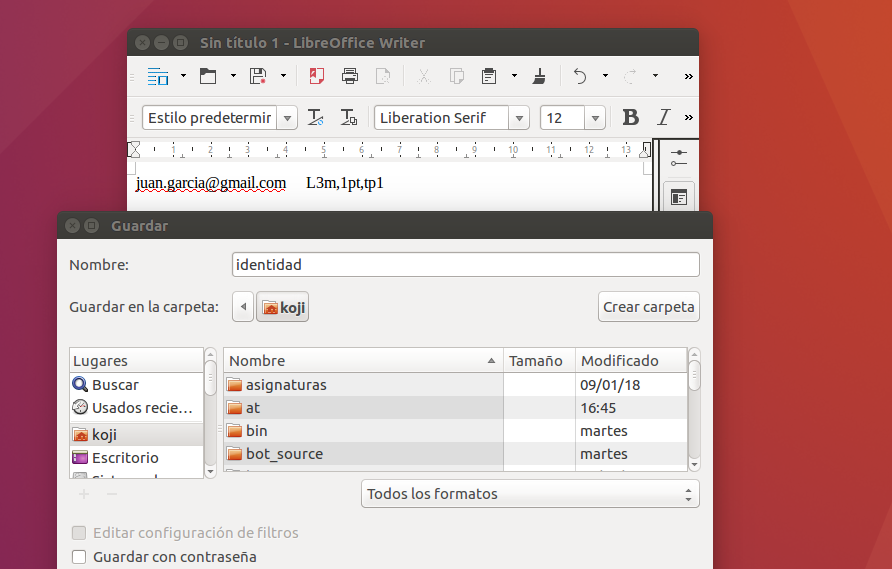
\includegraphics[width=0.8\textwidth]{images/libre01}
  \caption{Guardar fichero con contraseña en LibreOffice.}
  \label{fig:libre}
\end{figure}
    \item
Una herramienta de gestión de contraseñas. Por ejemplo, KeePassX
    \end{enumerate}


\subsection{Contraseña maestra}
Para las soluciones 3 y 4 del apartado anterior, es de vital importancia recordar una contraseña maestra, sin ella, habremos 
perdido el acceso a todas las demás. La ventaja fundamental es que se trata de una única contraseña. Una opción
es apuntar un recordatorio de contraseña. 

Ejemplo: partimos de una frase.
 \emph{Rascayú, cuando mueras que harás tú}. Usamos la contraseña \emph{R,cmqht?}. Y escribimos, en texto sin cifrar, el recordatorio de contraseña
\emph{canción de los años 40}.



\subsection{KeePassX}

KeePassX es una aplicación que permite guardar y gestionar nuestras contraseñas de manera razonablemente
segura. 
Es bastante
popular y se desarrollada activamente desde 2005 como software libre y gratuito. Por 
todo ello es razonable suponer que no tiene problemas
serios o puertas traseras, habrían sido detectados.
Está disponible para Microsoft Windows, Linux y MacOS.
Todas el contenido que añadamos se cifra con algoritmos estándar
de buena calidad, AES o Twofish con claves de 256 bits. 

Para guardar contraseñas de poco valor, por ejemplo de páginas web que
no sean especialmente importantes y que no usemos mucho, posiblemente
podemos confiar en la opción de autoguardado del navegador.
Pero para otros usos de mayor importancia, como nuestro correo principal,
bancos, trabajo, contraseñas del teléfono movil, etc, el uso de una
aplicación como KeePassX
es muy conveniente.

KeePassX tiene otra característica útil: la contraseñas se pueden
usar aunque estamos rodeados de personas que puedan ver nuestra pantalla,
puesto que permite copiar y pegar contraseñas sin mostrarlas. 
Si guardamos nuestras contraseñas en un documento de un procesador de
textos, no tenemos esta ventaja.



\subsubsection{Contraseña maestra y archivo llave}
Además de una contraseña maestra, KeePassX permite usar los denominados
\emph{archivos llave}. Es un concepto similar al de una llave mecánica
tradicional, algo que una persona necesita para acceder al sistema,
que puede ser copiado con relativa facilidad. Así, para poder acceder 
a las contraseñas, hace falta tener ese archivo llave, típicamente guardado
en un pendrive, en un cd, etc

Podemos configurar KeePassX para que sea necesario o bien la contraseña maestra,
o bien el archivo llave, o bien ambas cosas.

\subsubsection{Organización de KeePassX}

En KeePassX, el concepto de mayor orden jerárquico es el de
\emph{base de datos}. Es un fichero donde guardaremos nuestras contraseñas, todo
el contenido de este fichero estará cifrado con una única clave maestra. 
Un usuario individual normalmente tendrá una única base de datos, mientras
que en entornos donde haya contraseñas compartidas entre varios usuarios,
será normal emplear varias bases de datos, posiblemente una para individuo
y otra diferente para cada grupo.

Dentro de cada base de datos, se definen \emph{grupos} (de contraseñas).
Una organización típica sería tener por ejemplo un grupo para el ocio, otro
para el trabajo o estudios, prácticas, etc

Dentro de cada grupo, añadimos \emph{entradas}. Una entrada es una contraseña,
junto con otra información relacionada. En el apartado \emph{añadir entrada}
podemos añadir la siguiente información:

\begin{itemize}
\item
Título

Nombre que asignamos a la entrada.
\item
Nombre de usuario

\item
URL

\emph{Universal Resource Locator}. Una dirección web, la del sitio
donde se usa la contraseña.

\item
Expira

Por motivos de seguridad, es conveniente cambiar de vez en cuando las contraseñas.
Para ello, podemos indicar aquí una fecha de caducidad de la contraseña.
Cuando llegue ese momento, quedará marcada como caducada para recordar al
usuario que debería cambiarla, aunque no se borra de la base de datos.

\item
Notas

Es un espacio reservado para las anotaciones que nos parezcan convenientes.
\end{itemize}


En el apartado \emph{avanzado} podemos añadir:

\begin{itemize}
\item
Atributos adicionales

Similares a las notas, pero pueden ordenarse por categorías.

\item
Adjuntos

Permiten incluir cualquier fichero en la entrada. Un código QR, una tarjeta
de claves, etc.
\end{itemize}

\subsubsection{Uso de KeePassX}

Una vez que nos hayamos familiarizado con los conceptos básicos de esta aplicación,
su uso es muy sencillo. 


    \begin{enumerate}
    \item
Creamos una nueva base de datos, le asignamos contraseña y/o archivo llave.
(Figura \ref{fig:crea_bd})
\begin{figure}[htpb]
  \centering
    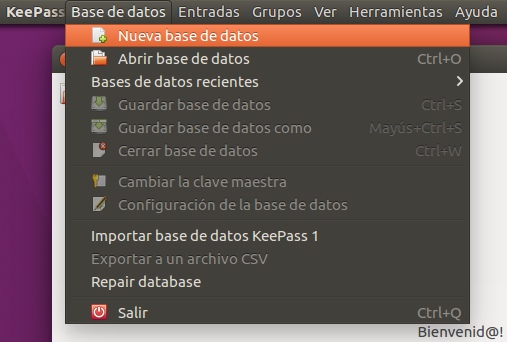
\includegraphics[width=0.8\textwidth]{images/kee01}
  \caption{Crear una nueva base de datos.}
  \label{fig:crea_bd}
\end{figure}

Este fichero deberíamos copiarlo en varios lugares, su pérdida puede
causarnos problemas muy severos.  Por ejemplo una copia en un pendrive
en casa y otra en un servicio de almecenamiento en la nube. Aunque alguien
acceda al fichero, no podrá consultarlo sin la contraseña. Tampoco nosotros.
    \item
Añádimos uno o más grupos 
(Figura \ref{fig:crea_gr}). Esto puede hacerse desde dos sitios

\begin{itemize}
\item
Menú \emph{grupos}, \emph{añadir grupos}.

\item
Haciendo clic con el botón secundario en el panel izquierdo, aparece un menú
contextual con la opción \emph{añadir nuevo grupo}.
\end{itemize}

\begin{figure}[htpb]
  \centering
    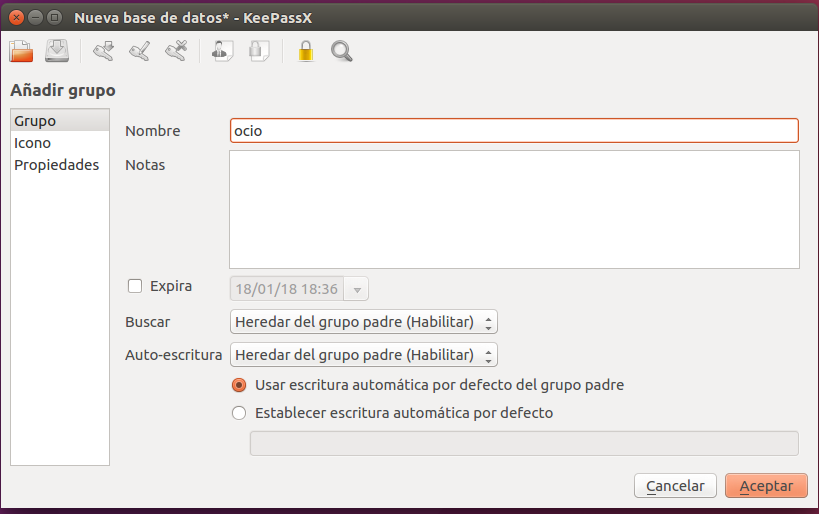
\includegraphics[width=0.8\textwidth]{images/kee02}
  \caption{Añadir un grupo.}
  \label{fig:crea_gr}
\end{figure}



    \item
Seleccionamos un grupo y añadimos entradas. 
(Figuras \ref{fig:kee3} y \ref{fig:kee4})
También podemos hacerlo desde dos sitios


\begin{itemize}
\item
Menú \emph{entradas}, \emph{añadir nueva entrada}

\item
Icono \emph{añadir nueva entrada}, (una flecha verde apuntando hacia 
una llave)
\end{itemize}

\begin{figure}[htpb]
  \centering
    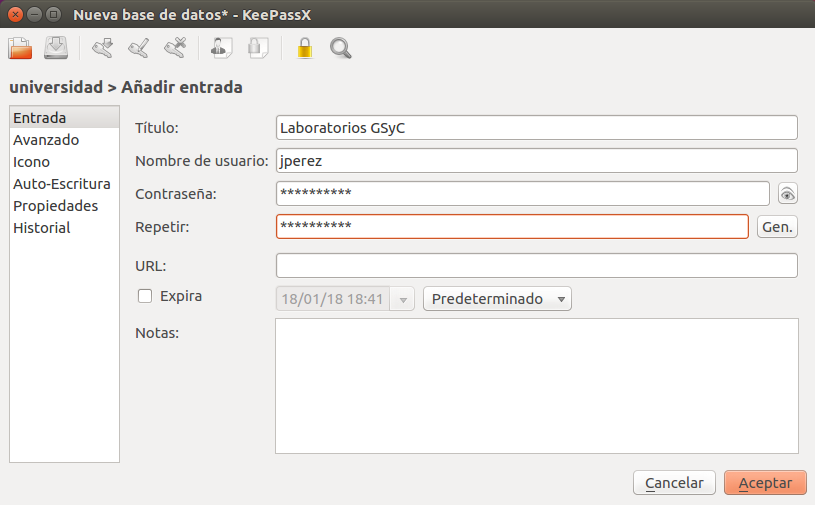
\includegraphics[width=0.8\textwidth]{images/kee03}
  \caption{Añadir una entrada. Campos básicos.}
  \label{fig:kee3}
\end{figure}


\begin{figure}[htpb]
  \centering
    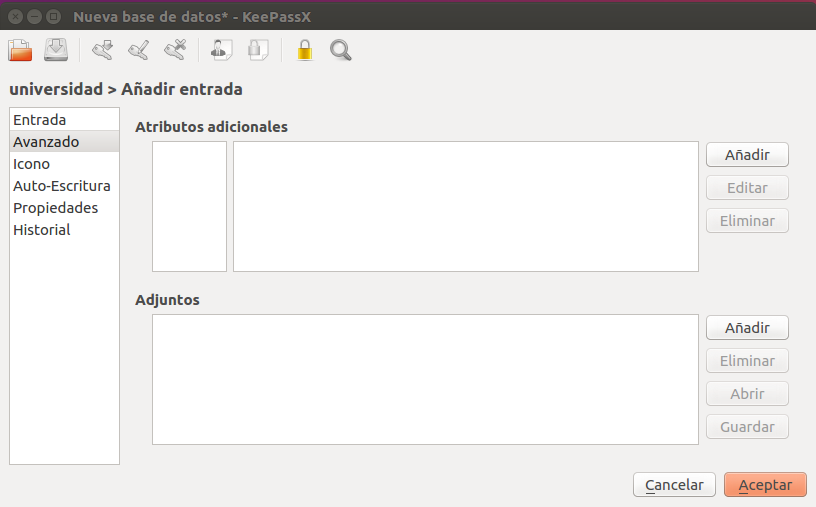
\includegraphics[width=0.8\textwidth]{images/kee04}
  \caption{Añadir una entrada. Campos avanzados.}
  \label{fig:kee4}
\end{figure}

Por omisión las contraseñas nunca se muestran en pantalla. Para verlas, pulsamos
en el icono que representa un ojo. También está disponible el botón \emph{gen},
que generará una contraseña aleatoria de calidad.
(Figura \ref{fig:kee3})

    \item
Una vez creadas las entradas, para usarlas basta hacer clic sobre la que necesitemos.
Recordando que podemos copiar y pegar, sin que la contraseña se llegue a ver en pantalla
\footnote{Esta opción no siempre funciona en Ubuntu 16.04, puede solucionarse instalando 
el paquete xsel:i386}.
(Figura \ref{fig:kee5})
\begin{figure}[htpb]
  \centering
    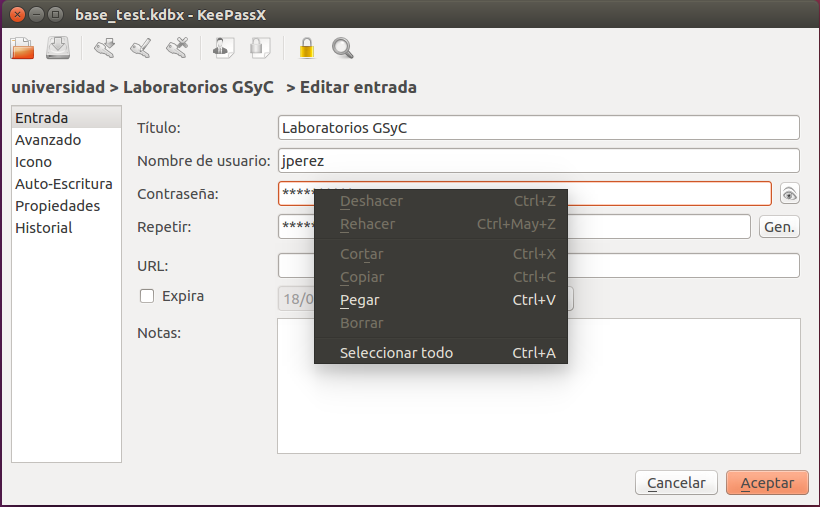
\includegraphics[width=0.8\textwidth]{images/kee05}
  \caption{Consultar una entrada.}
  \label{fig:kee5}
\end{figure}

    \end{enumerate}

\subsection{Ejercicios de gestión de contraseñas}


    \begin{enumerate}
    \item
Abre KeePassX. Para ello, pulsa en el teclado el botón \emph{meta} (el que tiene
el logo de Windows) y empieza a escribir la palabra \emph{keepassx}.

    \item
Crea una base de datos. Ponle el nombre que quieras, por ejemplo \emph{claves\_juan},
reemplezando \emph{Juan} por tu nombre. Ponle la contraseña maestra que quieras. Guárdala en el escritorio.

    \item
Guarda en el escritorio un documento de texto que se llame \emph{recordatorio}. Escribe dentro
un recordatorio de contraseña.

    \item
Crea dos o tres grupos de entradas. Con los nombres como por ejemplo \emph{ocio},  
\emph{universidad}, \emph{trabajo}, \emph{RedesSociales} o cualquier otro que te parezca 
adecuado.

    \item
Añade un total de 3 o 4 entradas a tu base de datos, repartidas entre los grupos
como te parezca bien. Al menos 2, que sean contraseñas reales de páginas web que 
uses realmente. El resto te las puedes inventar.

    \item
Ahora guarda la image de una tarjeta de coordenadas bancarias. Busca una cualquiera en google images,
usando las palabras \emph{tarjeta contraseñas} o mejor, \emph{password card}. 
Añádela a una nueva entrada.

    \item
Guarda la base de datos. Cierra KeePassX. Abrelo de nuevo. Comprueba que puedes
consultar las contraseñas y también la tarjeta.

    \item
Usa alguna de las contraseñas reales para entrar en un web, copiando y pegando,
sin que se llegue a ver en pantalla.

    \item
Recuerda que la cuenta de invitado que usas en el laboratorio es volátil, lo que has escrito
en el escritorio se borrará al salir. Seguramente querrás conservar tu base
de datos, en tal caso, envíatela por correo o guárdala en un pendrive si
has traido alguno, o en tu cuenta de almacenamiento en la nube si tienes alguna.


    \item
Ahora usarás una base de datos compartida con un compañero. Trabajad en grupos
de dos: alumno 1 y alumno 2. Si sois impares, excepcionalmente podéis ser tres.
En tal caso, que el alumno 3 haga lo mismo que el alumno 2. Si trabajas
solo, por ejemplo porque estás en casa, crea la base de datos igualmente y haz
el trabajo de los dos alumnos.

    \item
Alumno 1: prepara una nueva base de datos, para compartir por el grupo. Con el nombre que quieras. 
Con la contraseña maestra que quieras.

    \item
Alumno 1: escribe en el fichero \emph{recordatorio} un recordatorio también para esta nueva
base de datos.

    \item
Alumno 1: en la base de datos, añade un grupo de entradas. Añade 
una entrada o dos. Pueden ser inventadas.
Lo importante es que tengáis claro qué base de datos estáis usando en cada momento.

    \item
Alumno 1: dile la contraseña maestra al alumno 2. Envíale la base de datos al alumno 2 (sin el recordatorio). Puedes hacerlo de tres formas distintas, la que 
os venga mejor:

\begin{itemize}
\item
 Por correo, si ambos tenéis el correo a mano.

\item
Con un pedrive, si tenés alguno a mano

\item

Guardando el fichero en el ordenador. Tened en cuenta que
en la cuenta \emph{invitado}, el contenido del escritorio se borrará al cerrar la sesión. 
Para evitarlo:

\begin{enumerate}
\item
Alumno 1: usando el gestor de ficheros, copia la base de datos desde el escritorio hasta el disco \emph{equipo}, carpeta \emph{var}, subcarpeta \emph{tmp}

\item
Alumno 1: cierra tu sesión.

\item
Alumno 2: abre una sesión en el mismo ordenador.

\item
Alumno 2: arranca KeePassX y abre la base de datos, que seguirá en \emph{equipo}, carpeta \verb|/var/tmp|

\end{enumerate}

\end{itemize}




    \end{enumerate}


\section{Copias de seguridad}

\subsection{Problema de las copias de seguridad}
 
Otro de los principales problemas que tienen los usuarios de nuevas tecnologías es el de la copia
de seguridad de los datos. Los documentos se conservan en el disco duro del ordenador o en
el teléfono móvil. Cuando el dispositivo se estropea, le ataca un virus, se renueva, se pierde o su capacidad
se agota, hay un enorme riesgo de perder los datos. Es sorprendente la cantidad de personas
y empresas que gastan enormes cantidades de esfuerzo, tiempo y dinero en generar
contenidos digitales (informes, fotografías, grabaciones, cálculos, etc), sin preocuparse de custodiarlos
de manera mínimamente adecuada.

Los sistemas de almacenamiento en la nube como Dropbox, Microsoft OneDrive, iCloud, etc, resultan
una solución aceptable para muchos casos, pero con limitaciones serias:

\begin{itemize}
\item
Los datos permanecen fuera del contol del usuario. En caso de empresas, esto puede ser incluso contrario
a la ley.

\item
Para volúmenes elevados, resulta caro o incluso  inviable. Pensemos en fotografías o documentos gráficos de alta
resolución, grabaciones de audio, másters de vídeo, etc
\end{itemize}



En la actualidad los discos duros tienen mucha capacidad y son muy baratos. Son 
frágiles, pero podemos conseguir seguridad a partir de la redundancia: si guardamos 
datos en nuestro ordenador y en dos discos duros adicionales, a ser posible en ubicaciones
diferentes, tendremos una gran seguridad a un precio muy bajo.


El uso de discos internos SATA de 3.5 pulgadas  con 
\href
{https://tinyurl.com/ya4yfmyz}
{bases de conexión}
(\emph{docking station})
resulta especialmente conveniente.

\subsection{Sincronización de datos}

Tengo el disco duro lleno de material multimedia producido por mí. Hago una copia en un disco externo, tarda unas
pocas horas. La semana siguiente he generado material nuevo, que también quiero replicar. ¿Qué hago?

    \begin{enumerate}
    \item
Copio solo las novedades. Mala idea, es complicado llevar a mano la cuenta de qué ficheros son nuevos,
cuáles he retocado...

    \item
Lo copio todo otra vez. Mala idea, tarda mucho tiempo y fatigo el disco duro de manera innecesaria. Aumento la probabilidad
de que acabe fallando.

    \item
Solución correcta: usar una herramienta de sincronización. Por ejemplo, FreeFileSync. 

    \end{enumerate}



\subsection{FreeFileSync}
FreeFileSync es una aplicación de sincronización de ficheros. Es software libre y gratuito. Está disponible para Microsoft Windows, Linux y MacOS. 
Es un programa maduro, apareció en 2008 y desde entonces se sigue actualizando de manera continua. (Todo esto es muy importante para
decidir qué aplicación usar, para cualquier necesidad que tengamos)

Usaremos FreeFileSync para hacer una copia de tipo espejo de un sistema de ficheros a otro. Normalmente trabajaremos
desde un disco duro hasta otro diferente, por supuesto también podemos trabajar en distintas carpetas dentro
del mismo disco, pero por simplificar seguiremos hablando del \emph{disco original} y del \emph{disco espejo}.

El primer día que usemos el disco espejo, copiamos todos los directorios que nos interesen del original. Podemos usar
este programa o nuestro gestor de ficheros habitual. El segundo día y posteriores, usamos FreeFileSync para
que se copien al disco espejo solo los ficheros nuevos o actualizados.

\begin{figure}[htpb]
  \centering
    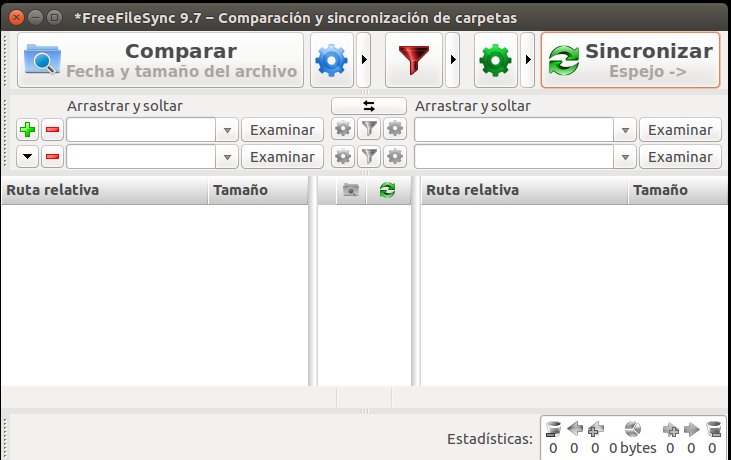
\includegraphics[width=0.8\textwidth]{images/ffs01}
  \caption{Pantalla principal de FreeFileSync.}
  \label{fig:ffs_main}
\end{figure}

En la ventana principal de FreeFileSync (Figura \ref{fig:ffs_main}) tenemos dos paneles con ficheros. En el de la izquierda, indicamos los directorios
del disco original que nos interesa respaldar.
En el de la derecha, los directorios del disco espejo donde se clonarán.
Seguiremos los pasos descritos a continuación.


    \begin{enumerate}
    \item
Configuramos la aplicación según nuestros requerimientos.
La configuración está dividida en tres ventanas:

\begin{itemize}
\item
\emph{Comparación}. (Figura \ref{fig:ffs_compara}). Icono de rueda dentada azul.
Las distintas opciones está autoexplicadas, normalmente no necesitaremos tocar nada.
\begin{figure}[htpb]
  \centering
    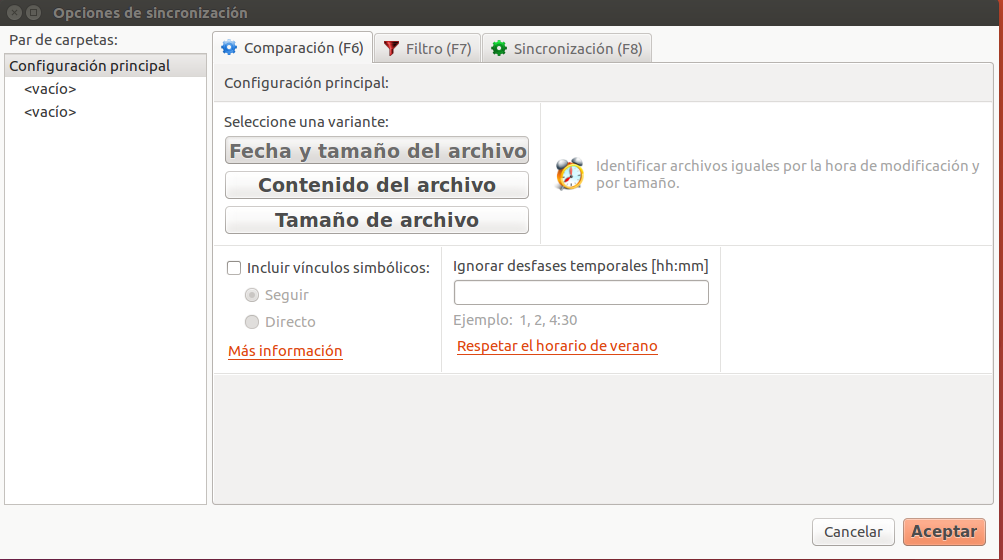
\includegraphics[width=0.8\textwidth]{images/ffs02}
  \caption{Comparación}
  \label{fig:ffs_compara}
\end{figure}

\item
\emph{Filtro}.(Figura \ref{fig:ffs_filtro}) Icono del embudo rojo. Aquí podemos indicar qué carpetas excluir, por ejemplo la carpeta
de la papelera de reciclaje, carpetas temporales o ficheros con copias de seguridad.

\begin{figure}[htpb]
  \centering
    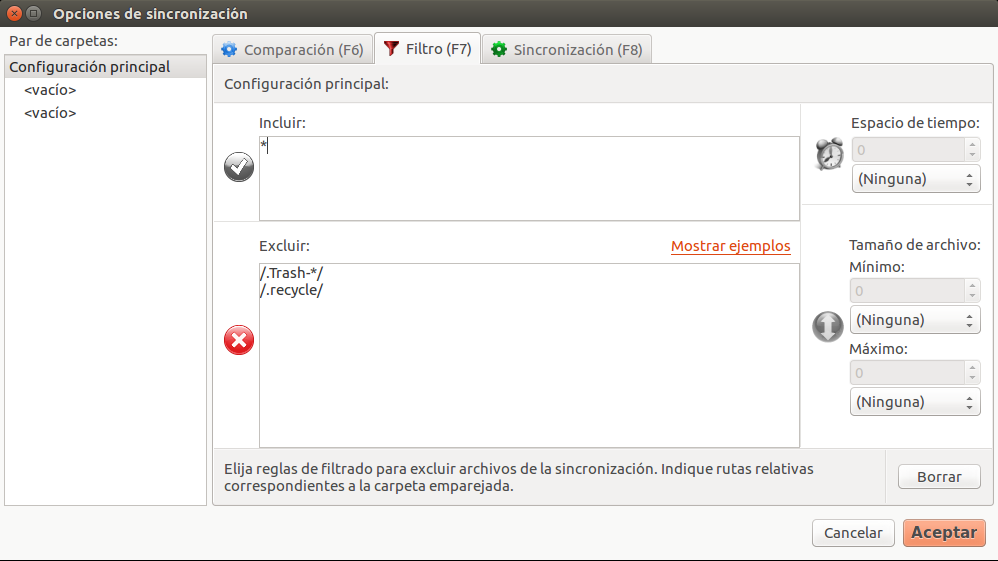
\includegraphics[width=0.8\textwidth]{images/ffs03}
  \caption{Filtro.}
  \label{fig:ffs_filtro}
\end{figure}

\item
\emph{Sincronización}. (Figura \ref{fig:ffs_sincro}) Icono de la rueda dentada verde. Esto sí es importante, porque por omisión
aparece en modo \emph{bidireccional}, que sirve para copiar ficheros desde el original al espejo
y desde el espejo al original. Pero esto no es lo que nos interesa en nuestro caso, queremos
que el espejo sea un clon del original. Para ello, tenemos que activar la opción \emph{espejo}.

\begin{figure}[htpb]
  \centering
    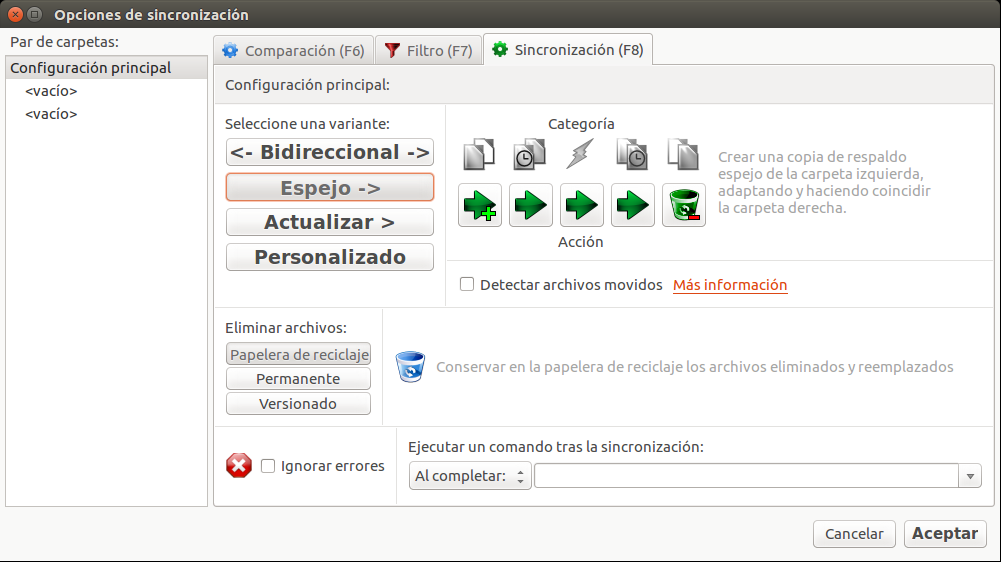
\includegraphics[width=0.8\textwidth]{images/ffs04}
  \caption{Sincronización }
  \label{fig:ffs_sincro}
\end{figure}
\end{itemize}


    \item
Añadimos al panel de la izquierda los directorios que nos
interesa sincronizar. En el panel de la derecha, indicamos los directorios donde queremos
que se guarden. El primer directorio de la izquierda se clonará en el primero de la derecha,
el segundo en el segundo, etc

    \item

Pulsamos el botón \emph{comparar}. Entonces la aplicación compará los directorios del panel
de la izquierda con los de la derecha, y nos indicará los pasos necesarios para el clonado.
De momento no hará nada, solo indicar.
Los ficheros a copiar tendrán una flecha verde. Los ficheros a modificar, una flecha con un signo
más. Los ficheros a borrar, una papelera. Con \emph{seleccionar vista}, podemos hacer
que solo se vean unos tipos de actualizaciones u otros

    \item
Si los cambios nos parecen correctos, pulsamos \emph{sincronizar}, con lo que la aplicación
actualizará todos los ficheros desde el original hasta el espejo.

    \item
Finalmente, guardaremos toda la configuración en un fichero de extensión \verb|.ffs_gui|, para
poder repetir el proceso en la siguiente ocasión,  sin volver a especificarlo todo.

    \end{enumerate}


\subsection{Ejercicios de sincronización de ficheros}

La sincronización de ficheros para hacer copias de seguridad normalmente la harás entre
dos discos disintos. Aquí usaremos dos carpetas, pero todo funcionará igual.

\begin{enumerate}
\item
Crea en el escritorio la carpeta \emph{datos}.

\item
Escribe dentro un fichero de texto, con el nombre que quieras y un par de líneas de texto de prueba.

\item
Ahora guardarás fotos en la carpeta
\emph{datos}. 
Supondremos que son los negativos digitales de fotos hechas
por tí. Para este tipo de fotos o vídeos, es conveniente organizar el trabajo por fechas, con un formato
parecido a este:

\verb|2018.04.07_fotos_viaje_cuenca|


\verb|2018.04.10_pruebas_camara_campus|


Observa que el uso de ceros a la izquierda de los números de un solo dígito. De esta forma, el orden
alfabético (que es el que usa normalmente el ordenador) coincide con el orden cronológico.

Crea un par de carpetas con un formato parecido a este y mete en cada una un par de fotos
que tengas a mano o que saques de cualquier web.


\item
Crea en el escritorio una carpeta llamada \emph{espejo}.


\item
Arranca FreeFileSync. Si no lo encuentras usando el botón \emph{meta} (el de windows), entonces arranca
una terminal de texto (pulsando Ctrl Alt T) y escribe \emph{KeePassX}

\item
Clona el contenido de \emph{datos} en \emph{espejo}.

\item
Guarda el archivo \verb|.ffs_gui| con la configuració de esta copia de seguridad en el escritorio. Ponle
el nombre que quieras. (pero no lo guardes ni dentro de 
\emph{datos} ni dentro de  \emph{espejo})


\item
Comprueba (a mano) que el directorio espejo ahora tiene lo mismo que el directorio de datos.


\item
Añade una línea de texto al fichero que escribiste en el apartado 2.4.2.


\item
Crea una nueva carpeta con fotos dentro de la carpeta 
\emph{datos}. Añade una nueva foto dentro.

\item
Abre el fichero \verb|.ffs_gui| que escribiste en el apartado 2.4.7. 

\item
Vuelve a sincronizar el fichero de datos en el espejo.

\item
Comprueba que el espejo se ha actualizado correctamente.

\end{enumerate}



\end{document}
